%\vspace{-2in}

\begin{figure}[H]
\centering
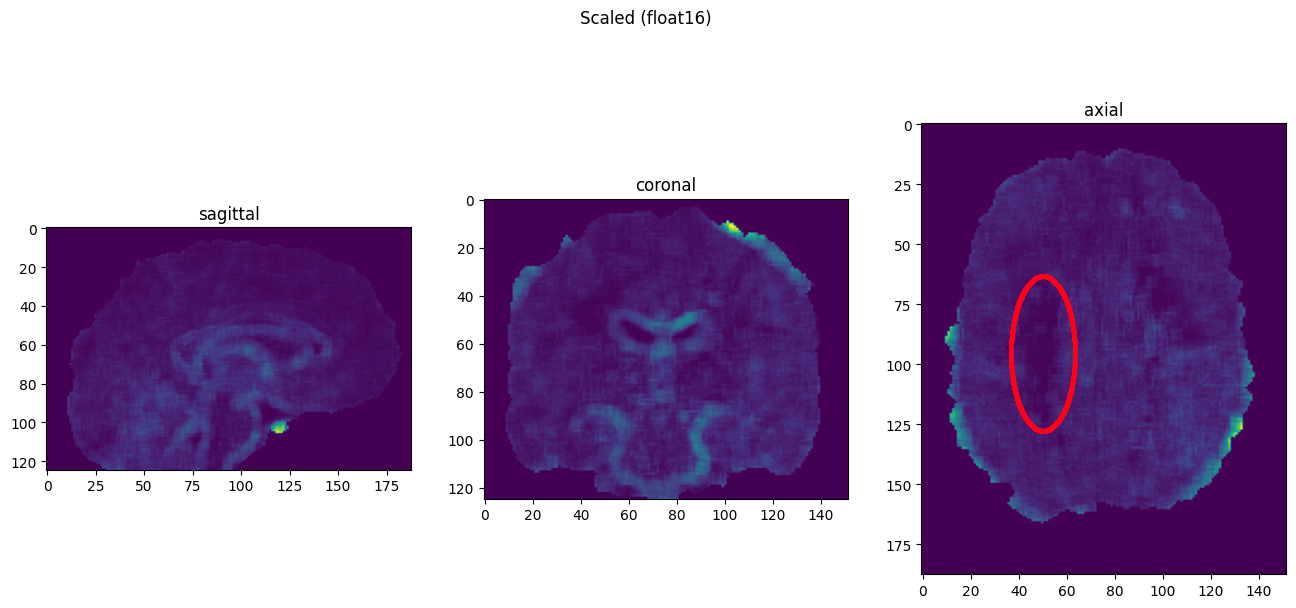
\includegraphics[width=0.9\textwidth]{rad_gldm_small_scale_16}
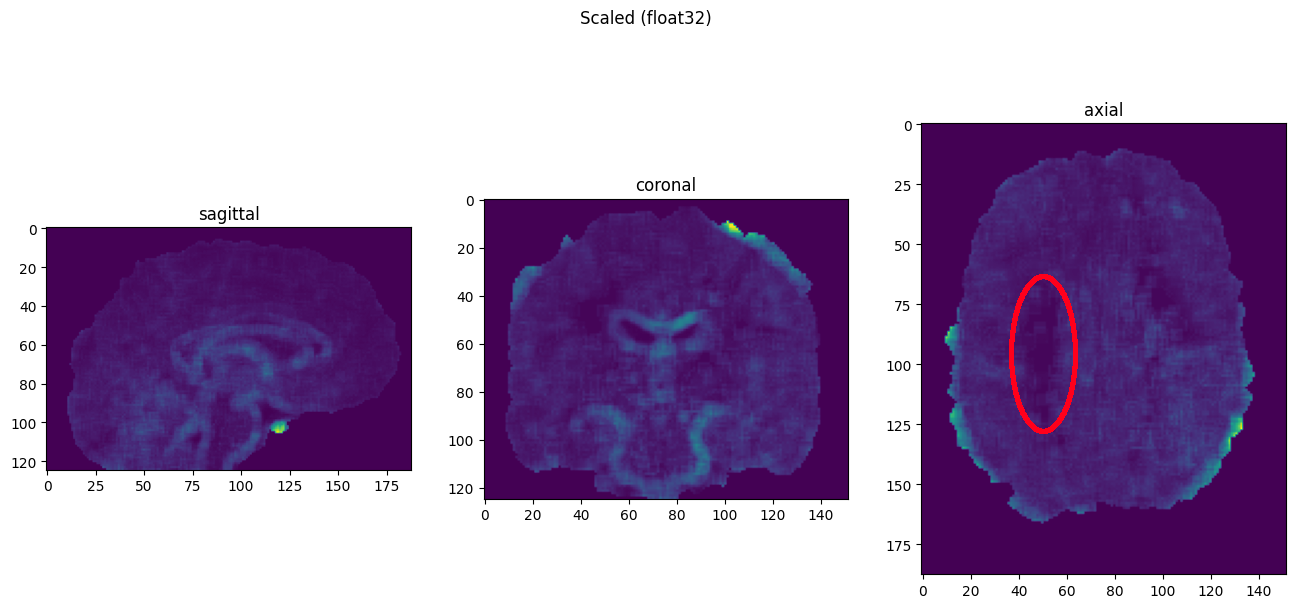
\includegraphics[width=0.9\textwidth]{rad_gldm_small_scale_32}
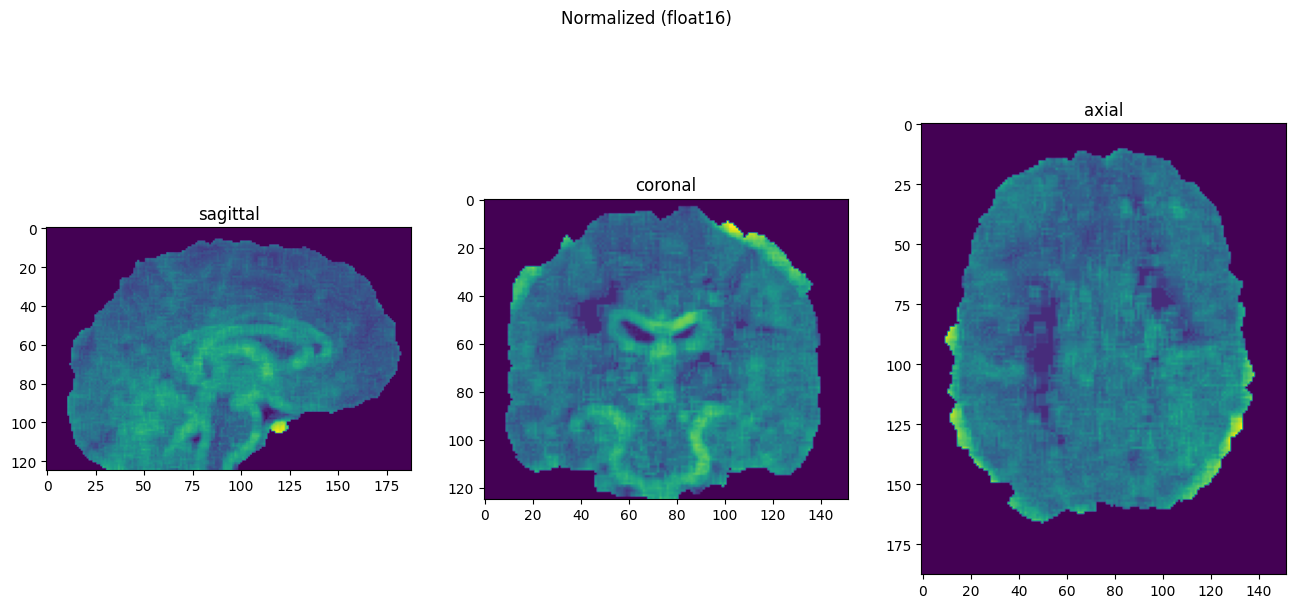
\includegraphics[width=0.9\textwidth]{rad_gldm_small_norm_16}
\caption{Slice: GLDM Small Dependence High Gray Level Emphasis}
\label{fig:gls}
\end{figure}

\begin{figure}[H]
\centering
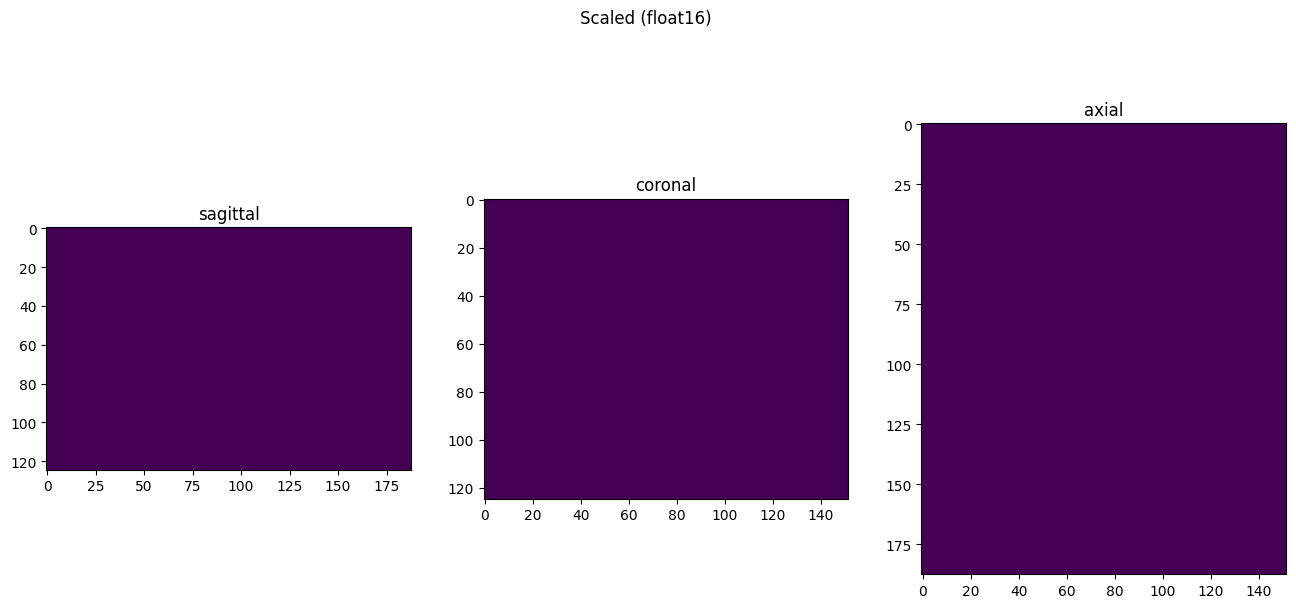
\includegraphics[width=0.9\textwidth]{rad_ngtdm_busyness_scale_16}
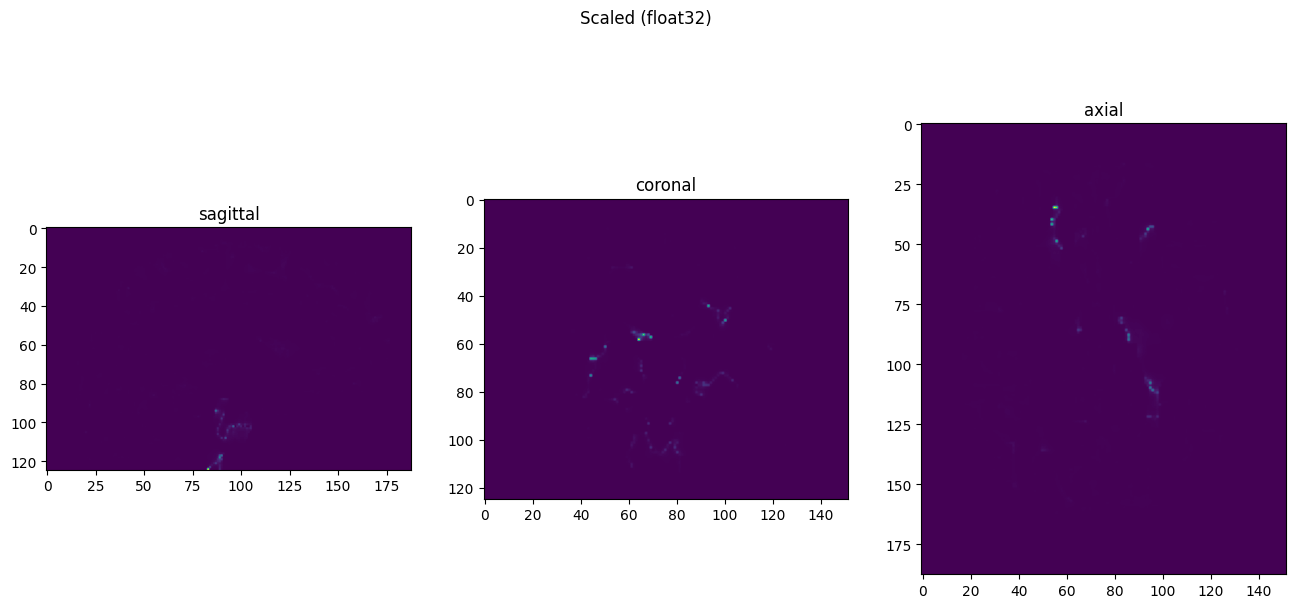
\includegraphics[width=0.9\textwidth]{rad_ngtdm_busyness_scale_32}
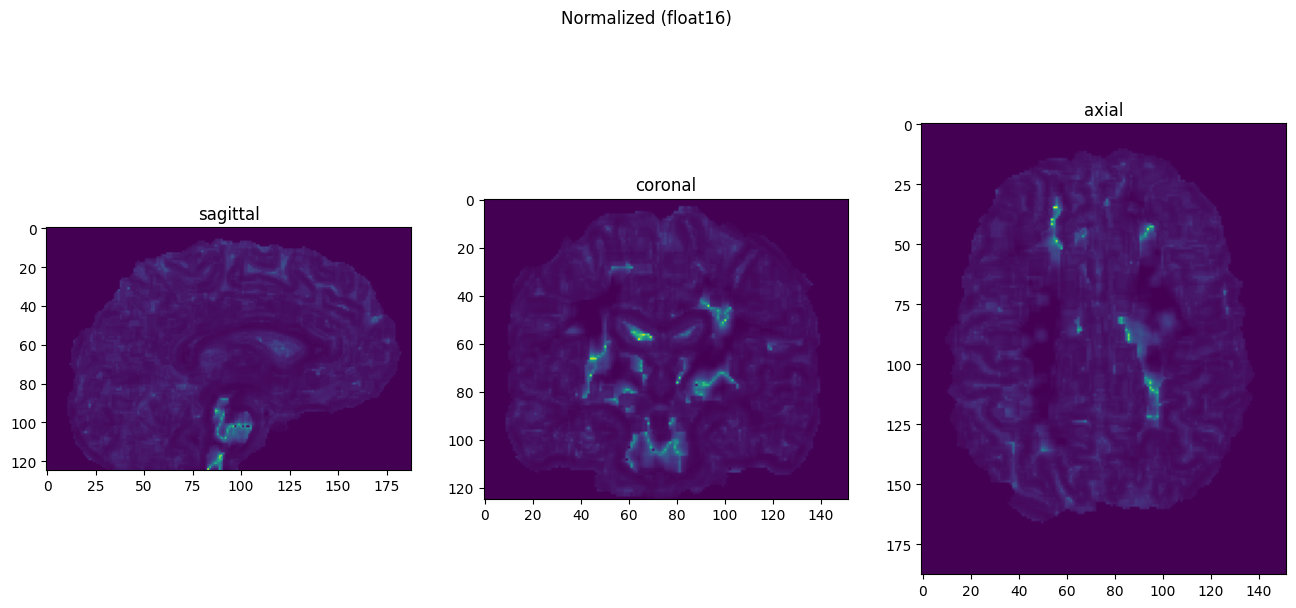
\includegraphics[width=0.9\textwidth]{rad_ngtdm_busyness_norm_16}
\caption{Slice: NGTDM Busyness}
\label{fig:ngb}
\end{figure}

\begin{figure}[H]
\centering
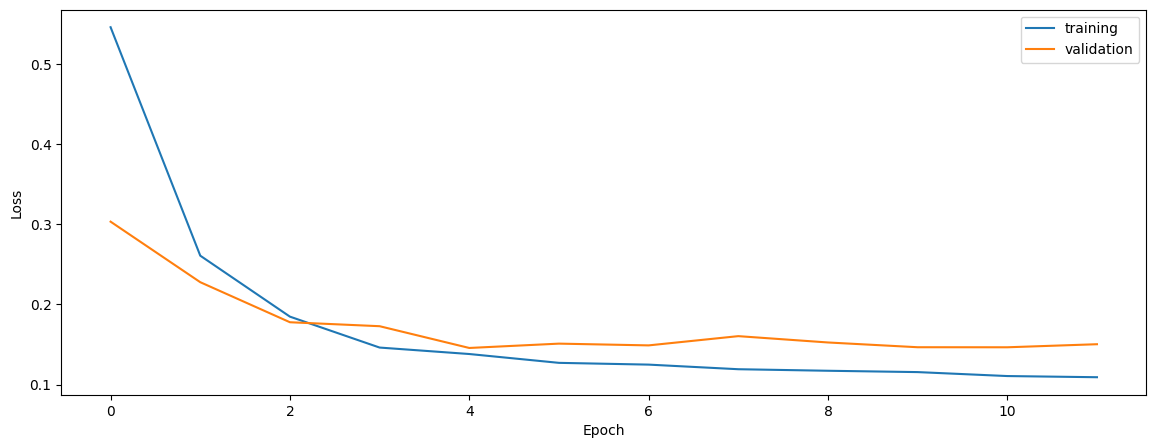
\includegraphics[width=0.7\textwidth]{subcortical_curve}
\caption{Training Curve: Subcortical}
\label{fig:curve-sub}
\end{figure}

\begin{figure}[H]
\centering
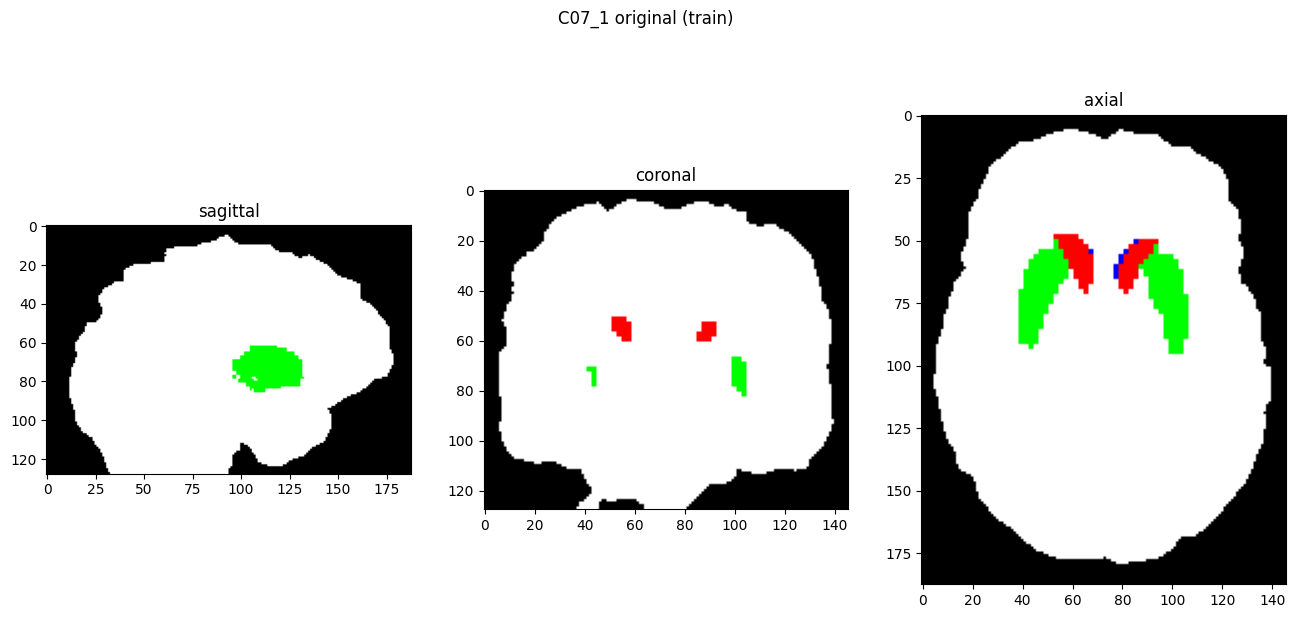
\includegraphics[width=0.9\textwidth]{subcortical_train_o}
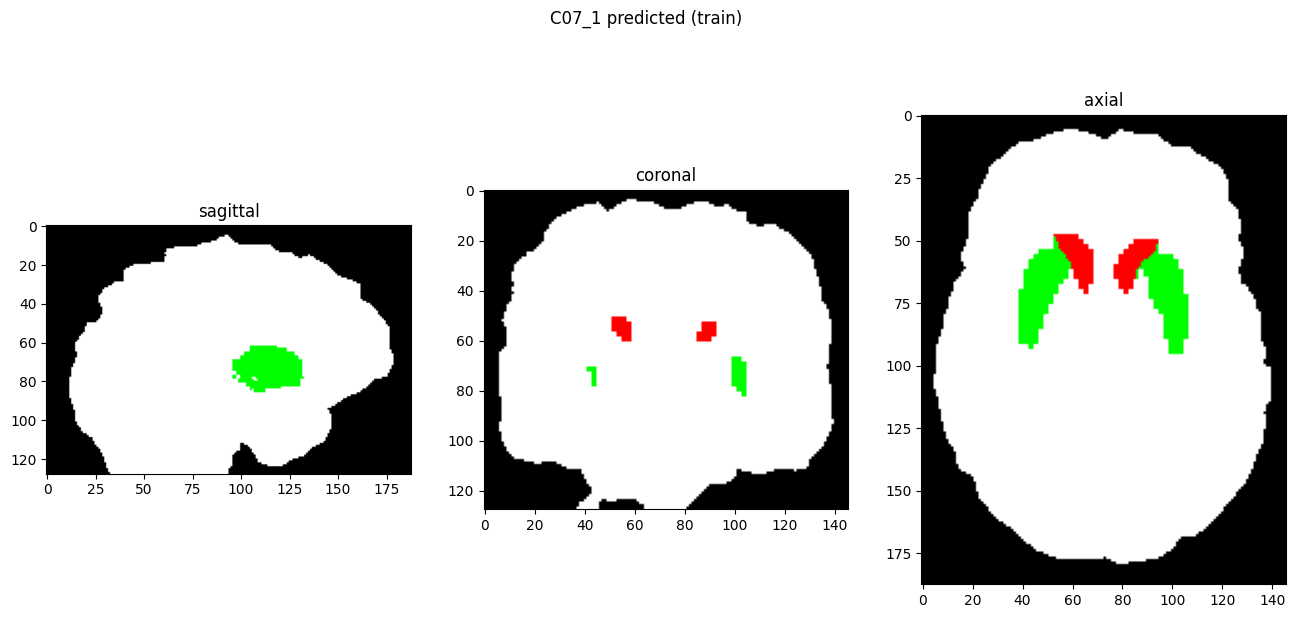
\includegraphics[width=0.9\textwidth]{subcortical_train_p}
\caption{Train Predictions: Subcortical}
\label{fig:pred-tra-sub}
\end{figure}

\begin{figure}[H]
\centering
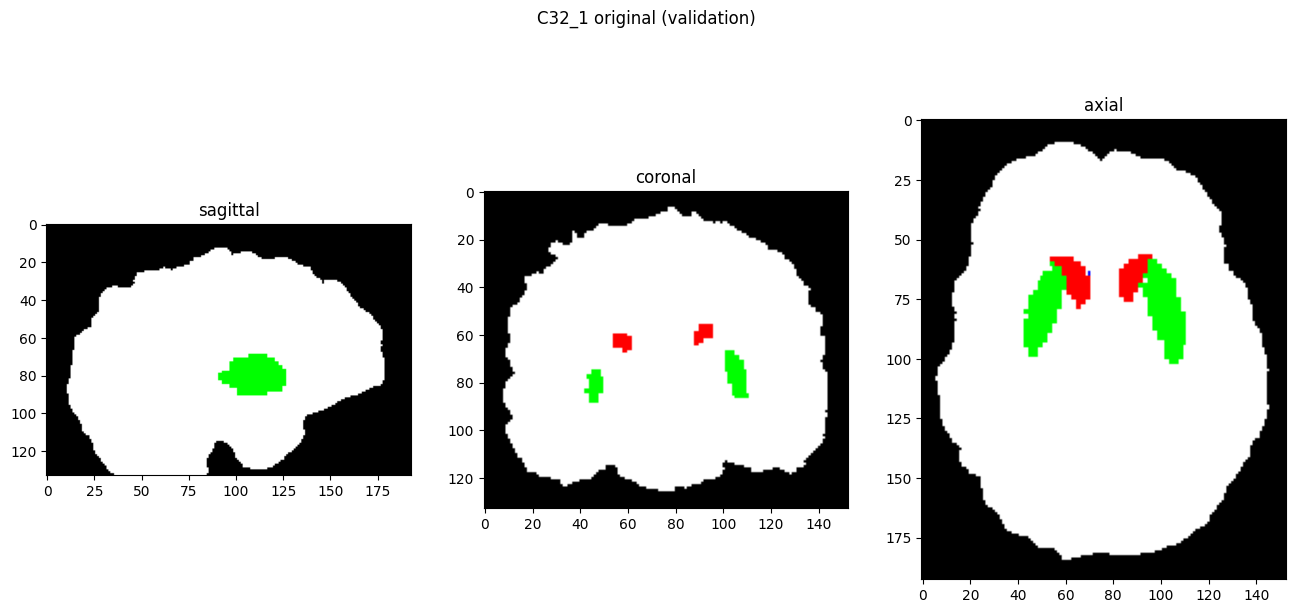
\includegraphics[width=0.9\textwidth]{subcortical_val_o}
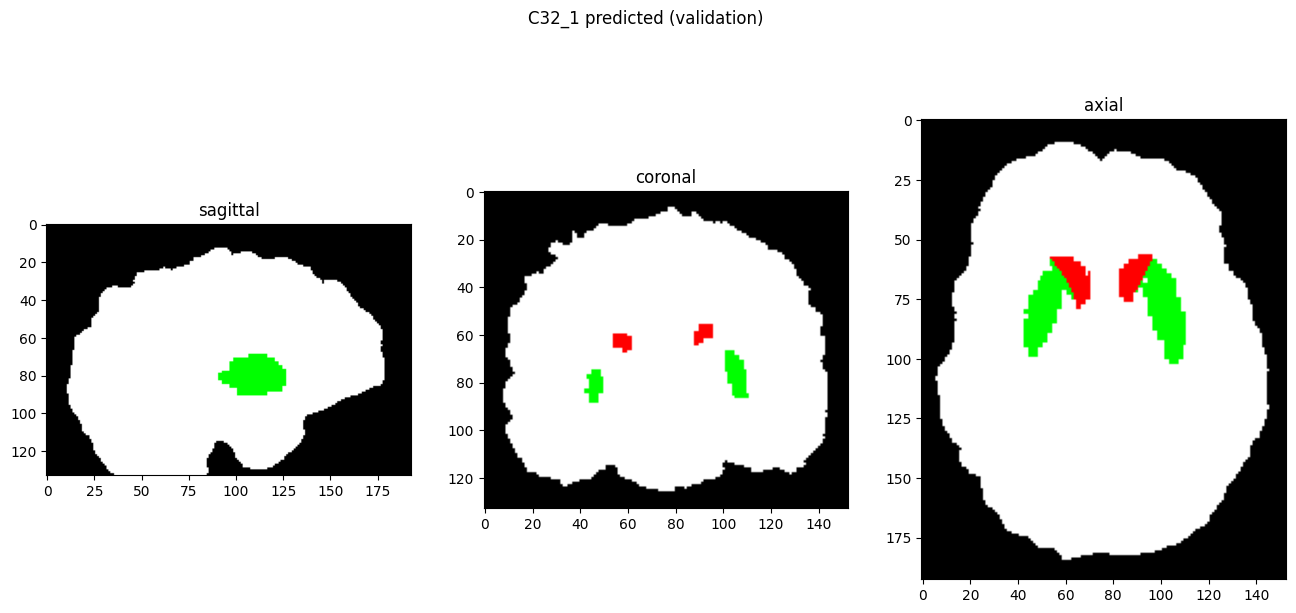
\includegraphics[width=0.9\textwidth]{subcortical_val_p}
\caption{Validation Predictions: Subcortical}
\label{fig:pred-val-sub}
\end{figure}

\begin{figure}[H]
\centering
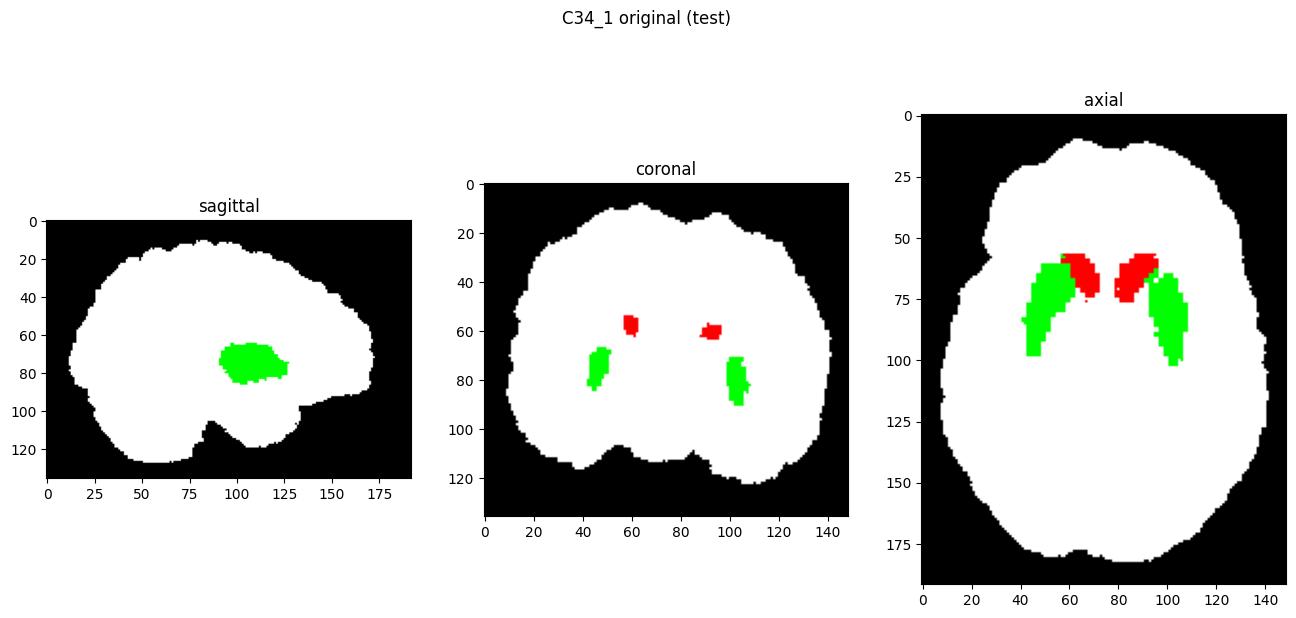
\includegraphics[width=0.9\textwidth]{subcortical_test_o}
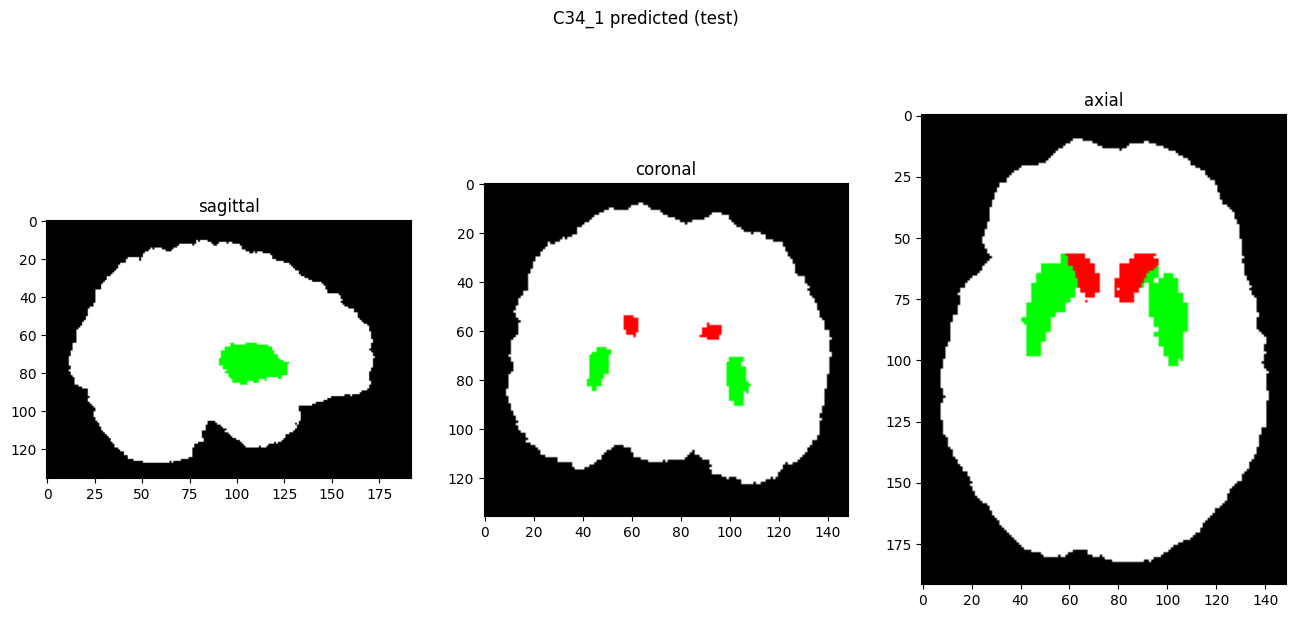
\includegraphics[width=0.9\textwidth]{subcortical_test_p}
\caption{Test Predictions: Subcortical}
\label{fig:pred-tes-sub}
\end{figure}

\begin{figure}[H]
\centering
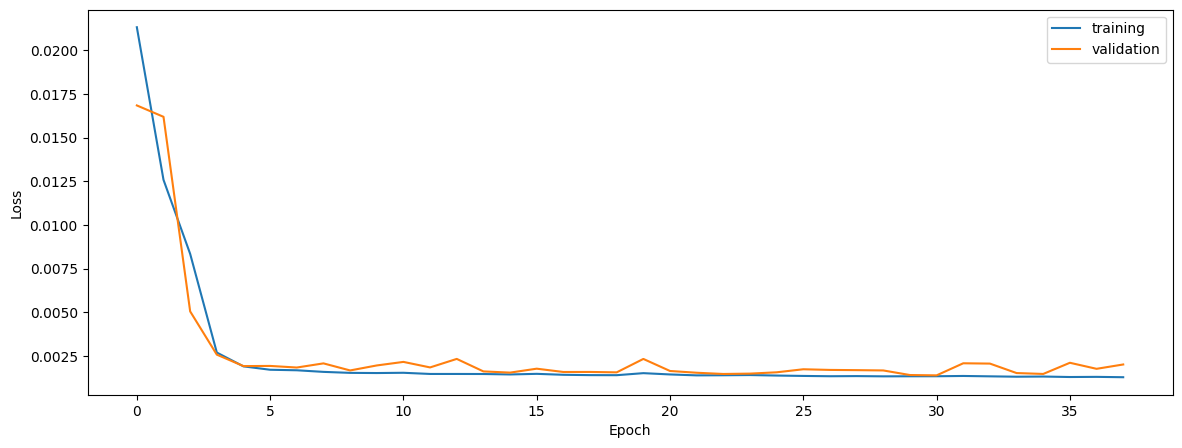
\includegraphics[width=0.7\textwidth]{md_curve}
\caption{Training Curve: Mean Diffusivity}
\label{fig:curve-md}
\end{figure}

\begin{figure}[H]
\centering
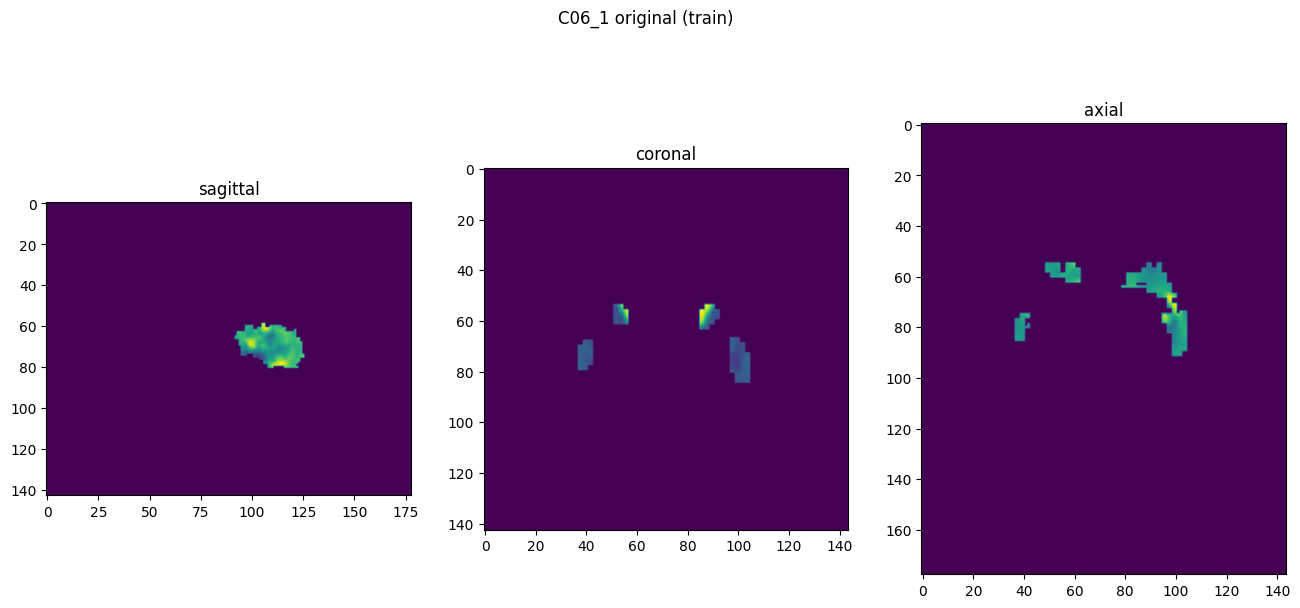
\includegraphics[width=0.9\textwidth]{md_train_o}
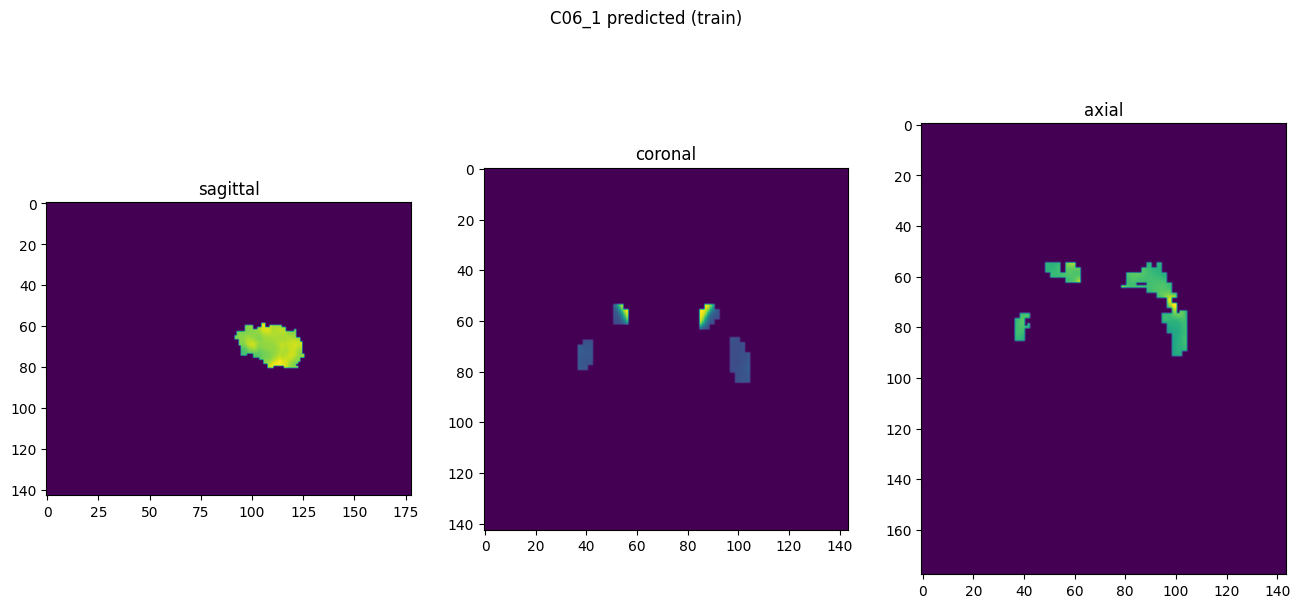
\includegraphics[width=0.9\textwidth]{md_train_p}
\caption{Train Predictions: Mean Diffusivity}
\label{fig:pred-tra-md}
\end{figure}

\begin{figure}[H]
\centering
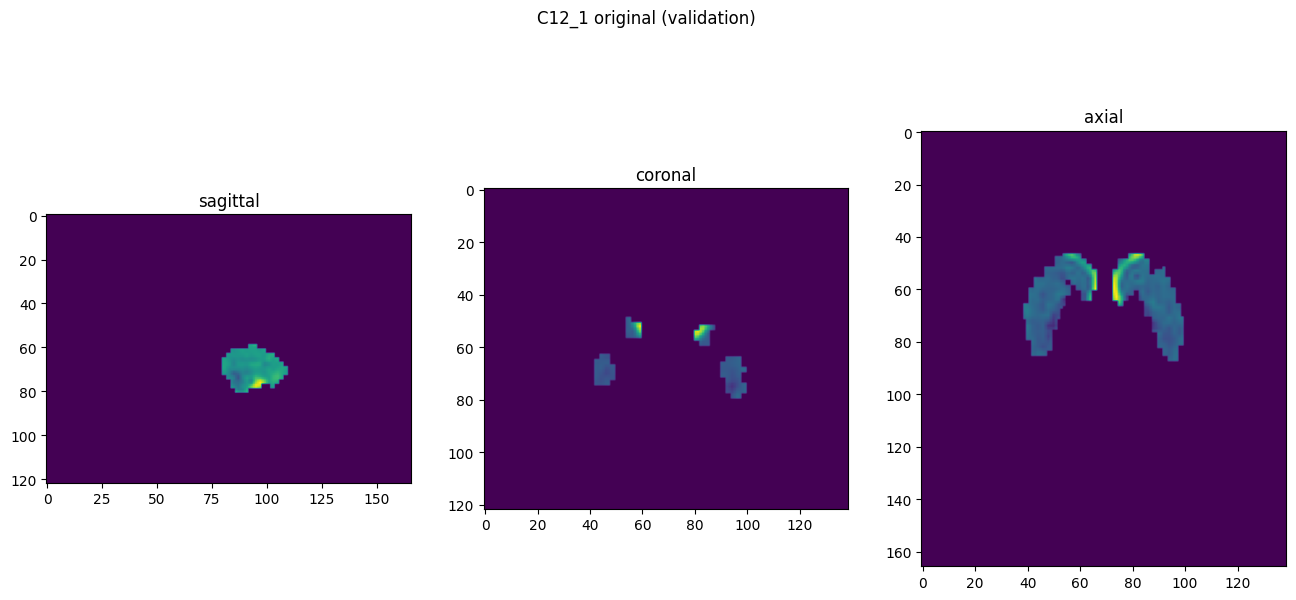
\includegraphics[width=0.9\textwidth]{md_val_o}
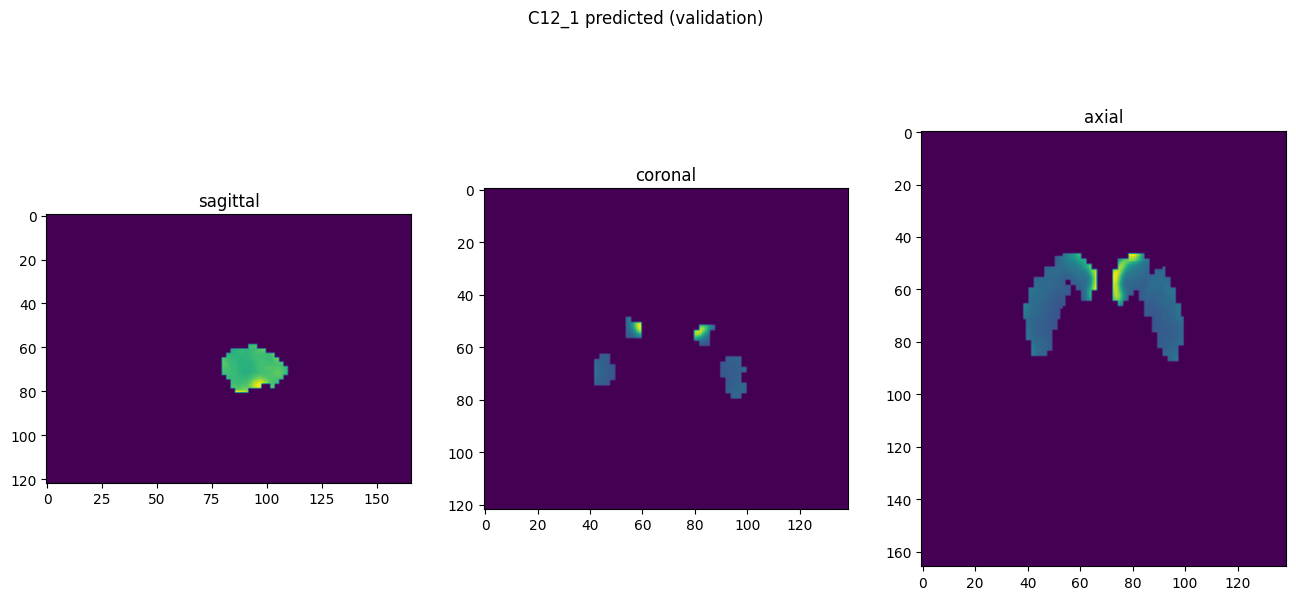
\includegraphics[width=0.9\textwidth]{md_val_p}
\caption{Validation Predictions: Mean Diffusivity}
\label{fig:pred-val-md}
\end{figure}

\begin{figure}[H]
\centering
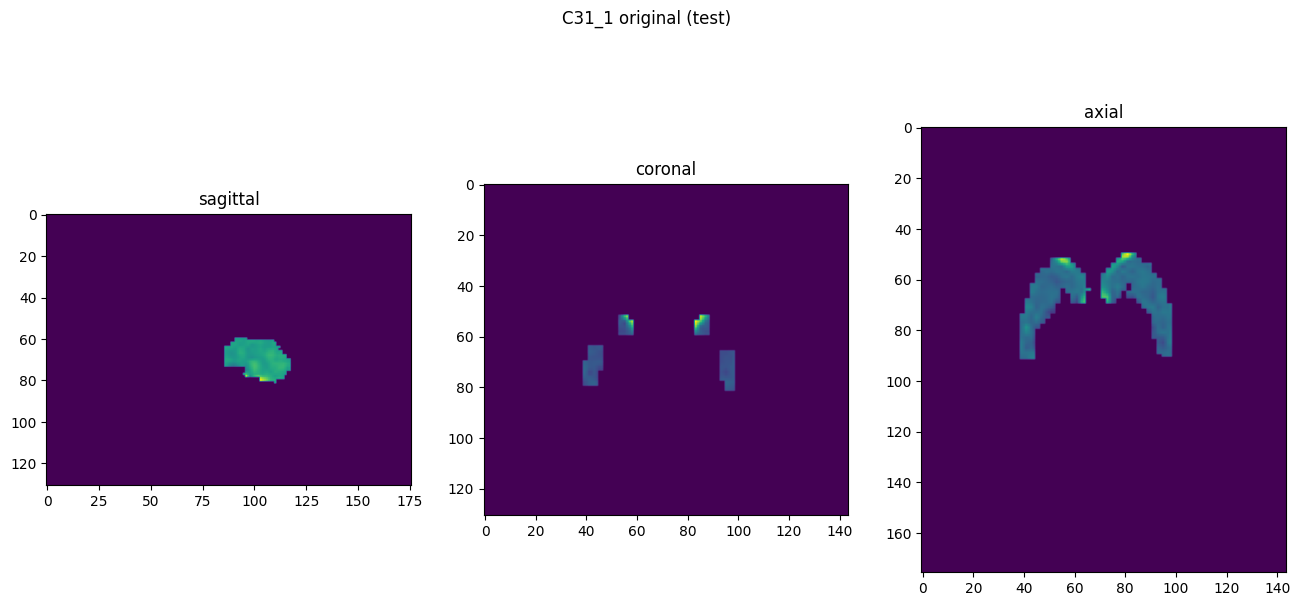
\includegraphics[width=0.9\textwidth]{md_test_o}
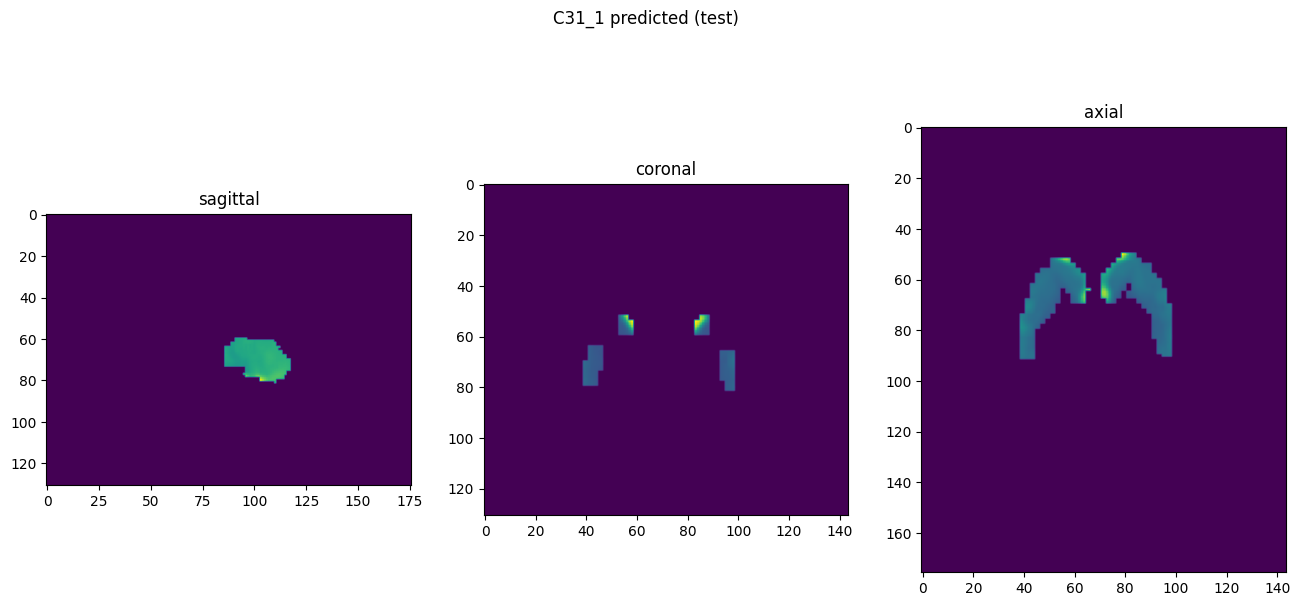
\includegraphics[width=0.9\textwidth]{md_test_p}
\caption{Test Predictions: Mean Diffusivity}
\label{fig:pred-tes-md}
\end{figure}

\begin{figure}[H]
\centering
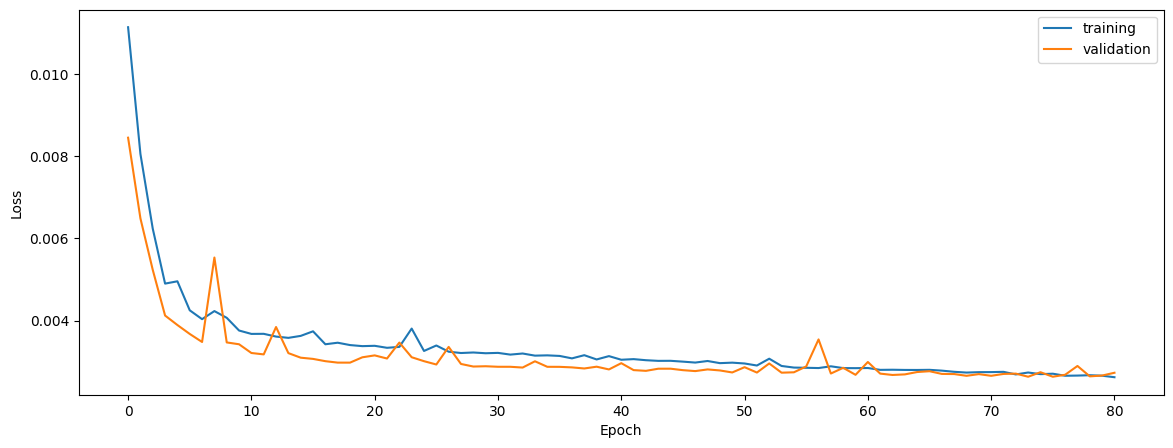
\includegraphics[width=0.7\textwidth]{fa_curve}
\caption{Training Curve: Diffusion Fractional Anisotropy}
\label{fig:curve-fa}
\end{figure}

\begin{figure}[H]
\centering
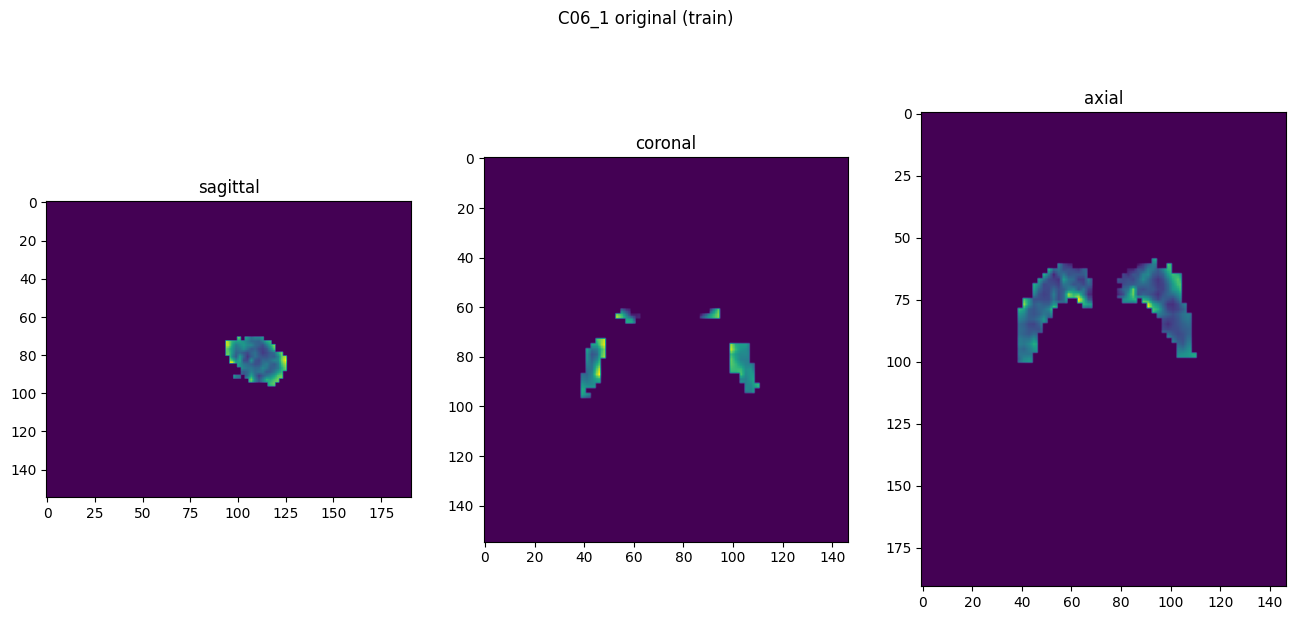
\includegraphics[width=0.9\textwidth]{fa_train_o}
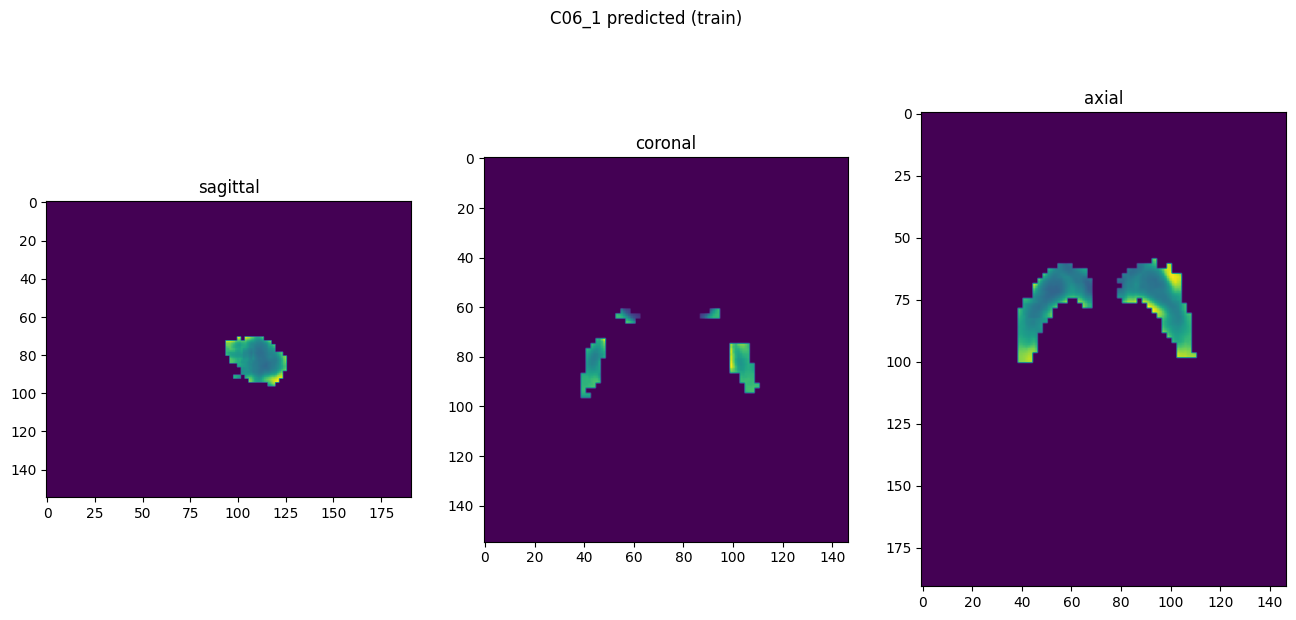
\includegraphics[width=0.9\textwidth]{fa_train_p}
\caption{Train Predictions: Diffusion Fractional Anisotropy}
\label{fig:pred-tra-fa}
\end{figure}

\begin{figure}[H]
\centering
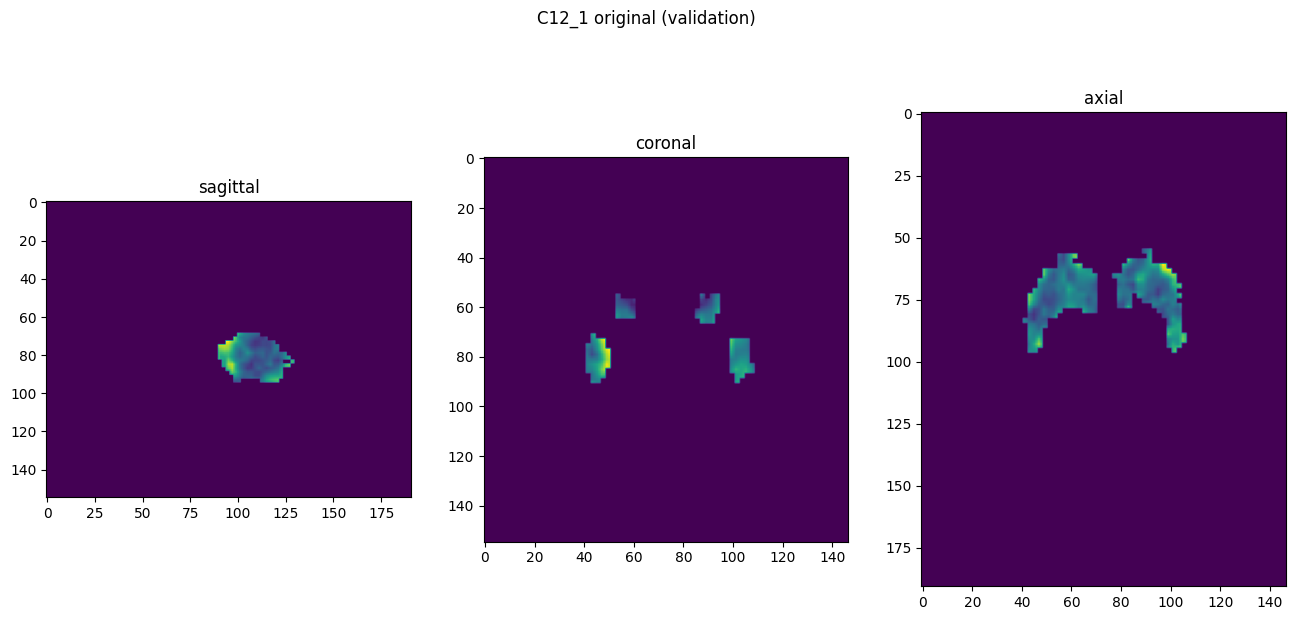
\includegraphics[width=0.9\textwidth]{fa_val_o}
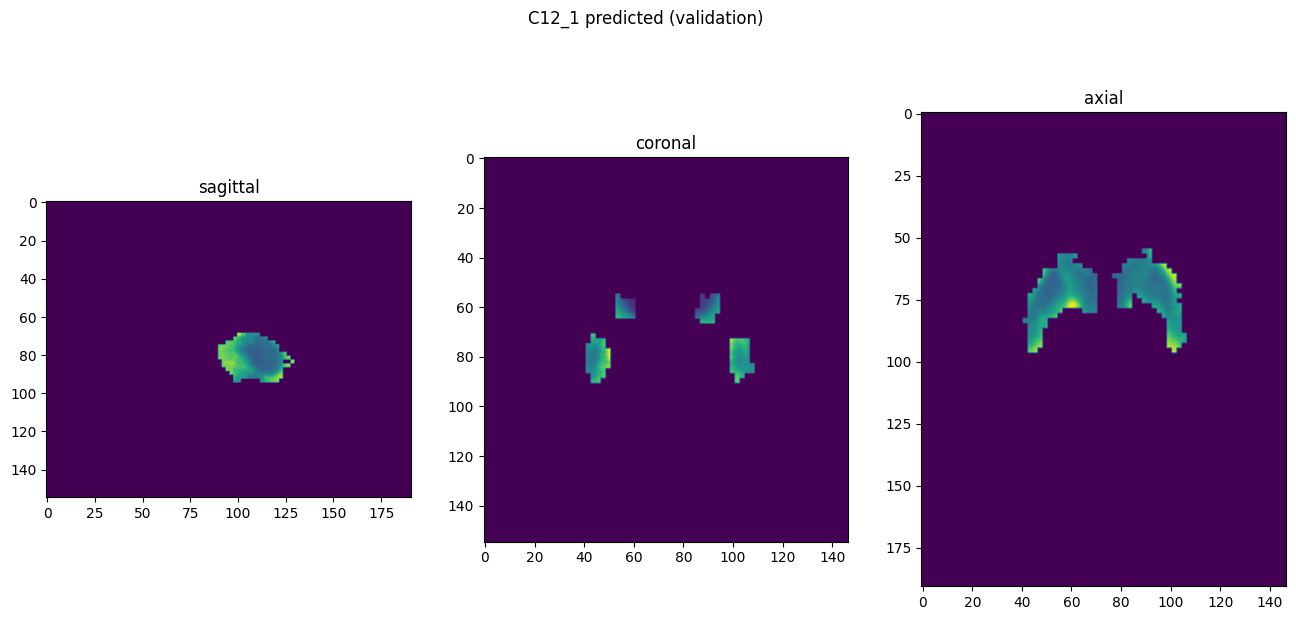
\includegraphics[width=0.9\textwidth]{fa_val_p}
\caption{Validation Predictions: Diffusion Fractional Anisotropy}
\label{fig:pred-val-fa}
\end{figure}

\begin{figure}[H]
\centering
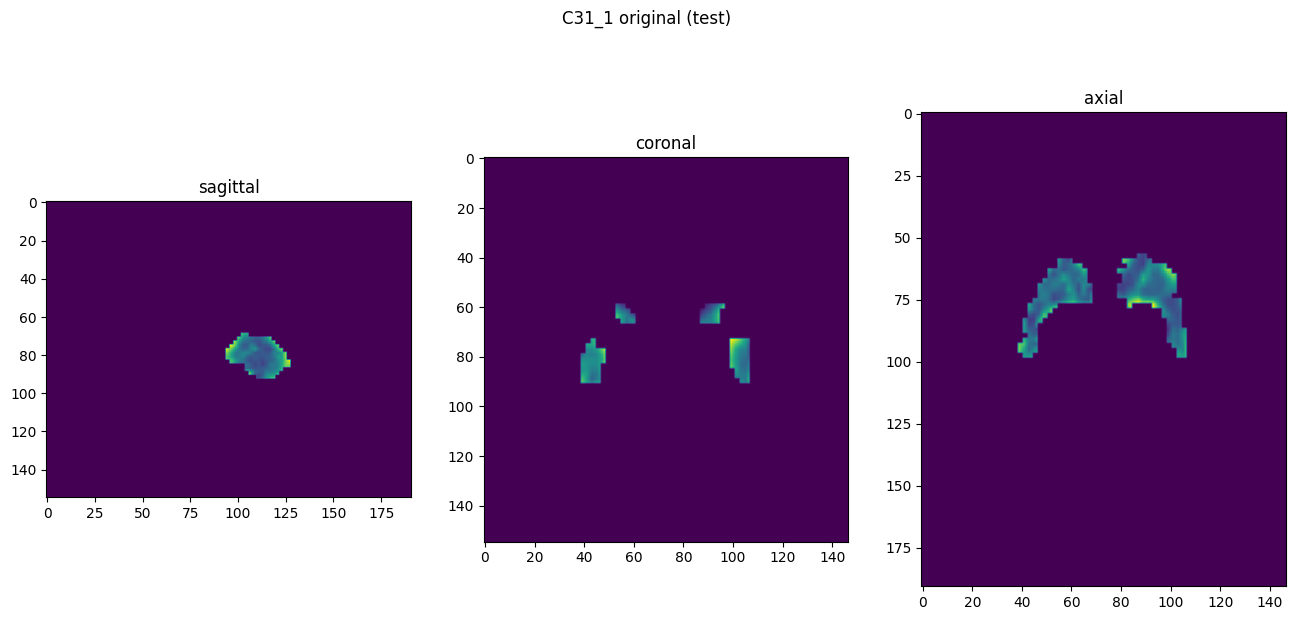
\includegraphics[width=0.9\textwidth]{fa_test_o}
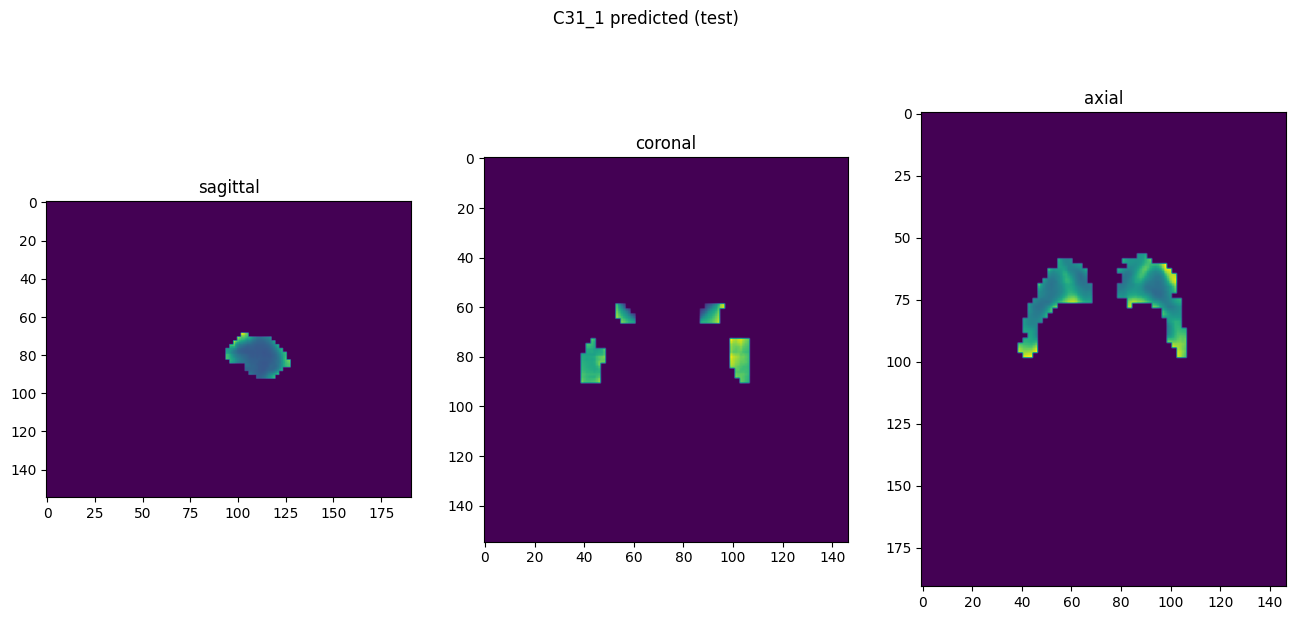
\includegraphics[width=0.9\textwidth]{fa_test_p}
\caption{Test Predictions: Diffusion Fractional Anisotropy}
\label{fig:pred-tes-fa}
\end{figure}

\begin{figure}[H]
\centering
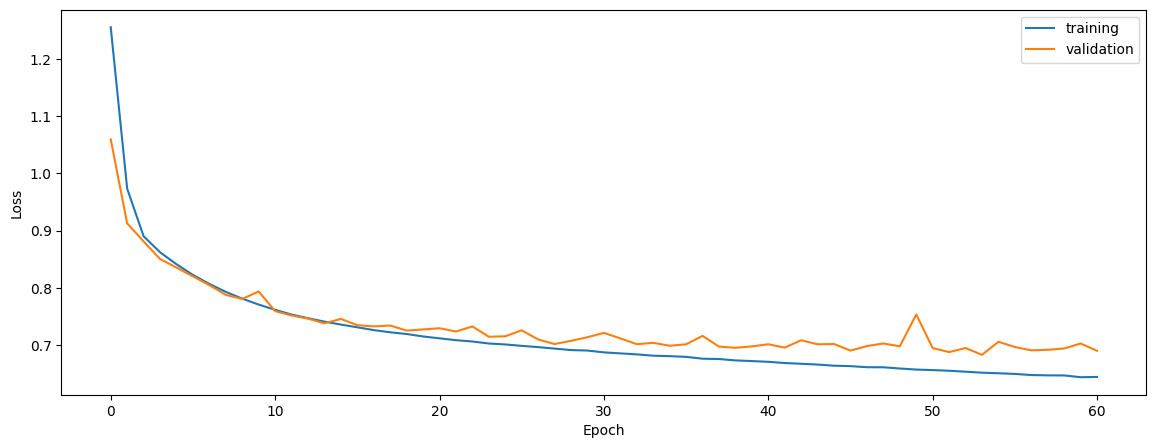
\includegraphics[width=0.7\textwidth]{con_curve}
\caption{Training Curve: Relative Connectivity}
\label{fig:curve-con}
\end{figure}

\begin{figure}[H]
\centering
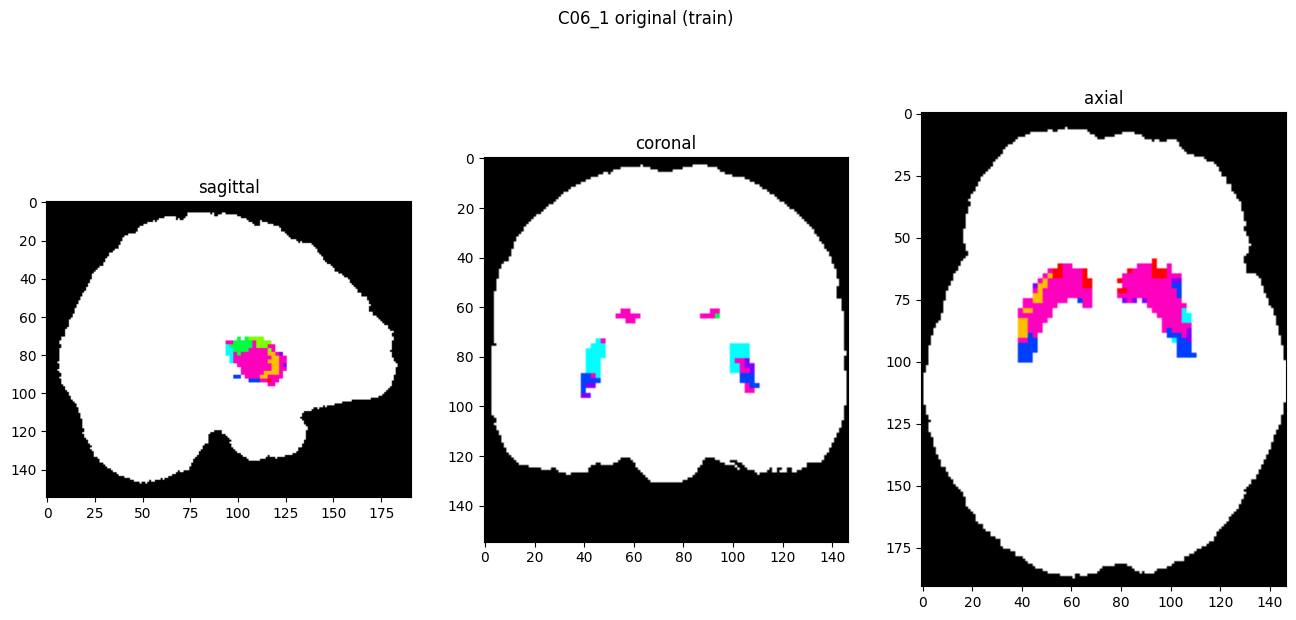
\includegraphics[width=0.9\textwidth]{con_train_o}
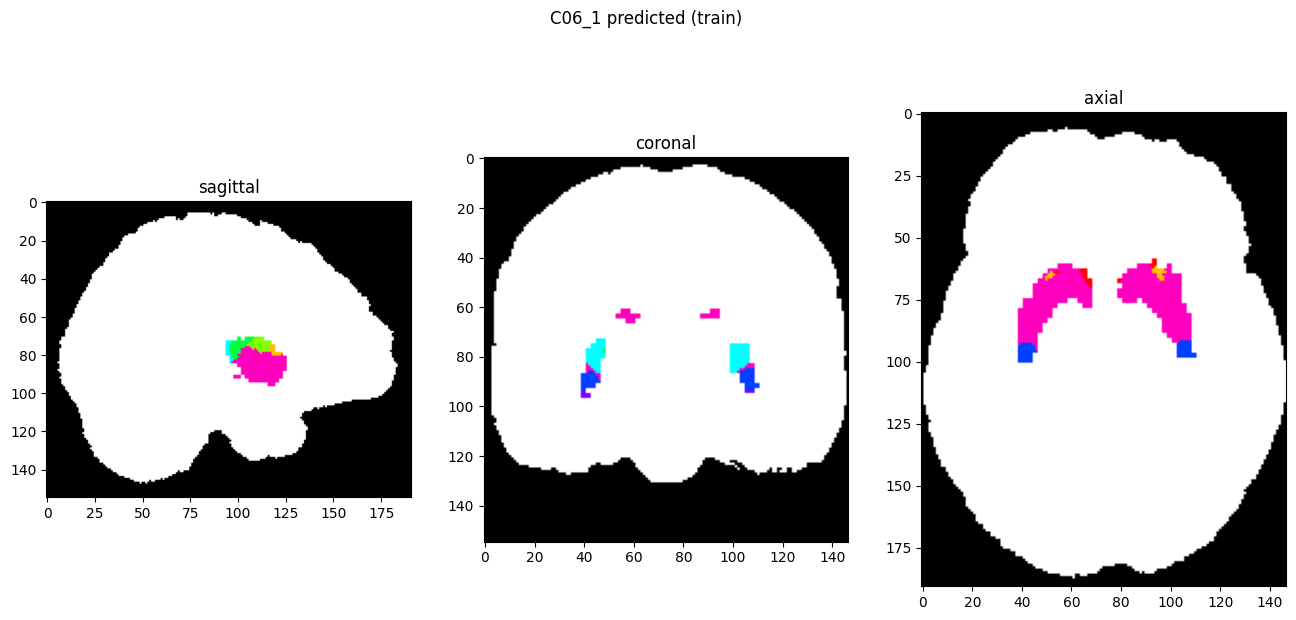
\includegraphics[width=0.9\textwidth]{con_train_p}
\caption{Train Predictions: Relative Connectivity}
\label{fig:pred-tra-con}
\end{figure}

\begin{figure}[H]
\centering
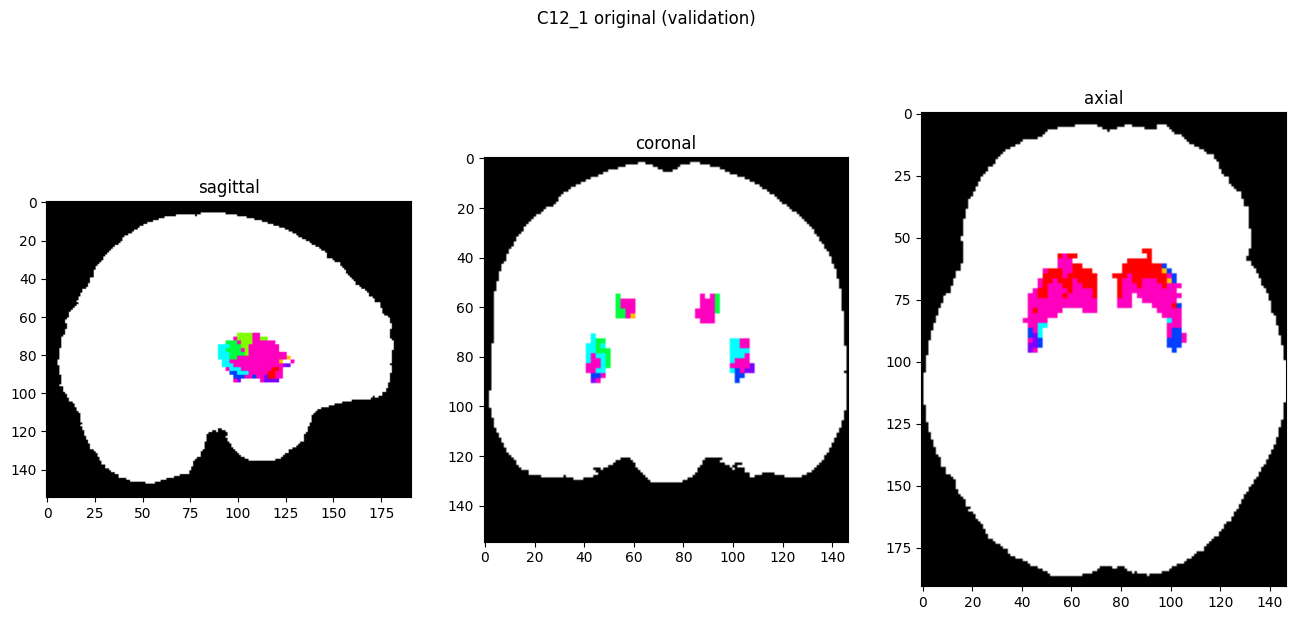
\includegraphics[width=0.9\textwidth]{con_val_o}
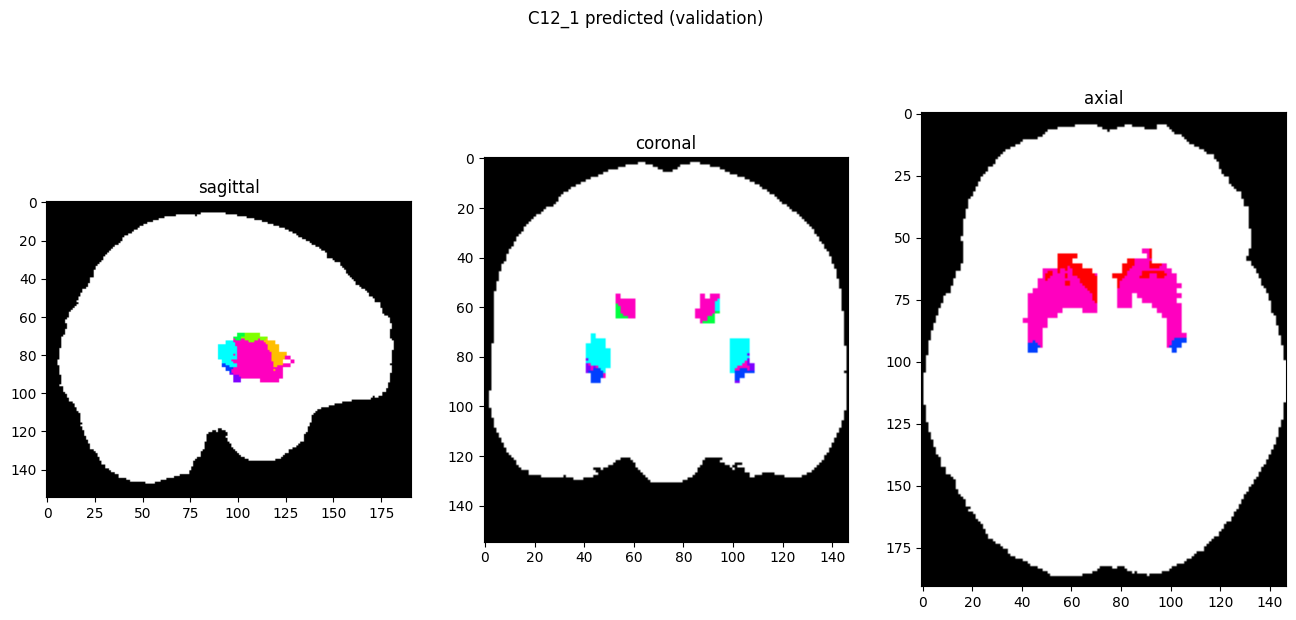
\includegraphics[width=0.9\textwidth]{con_val_p}
\caption{Validation Predictions: Relative Connectivity}
\label{fig:pred-val-con}
\end{figure}

\begin{figure}[H]
\centering
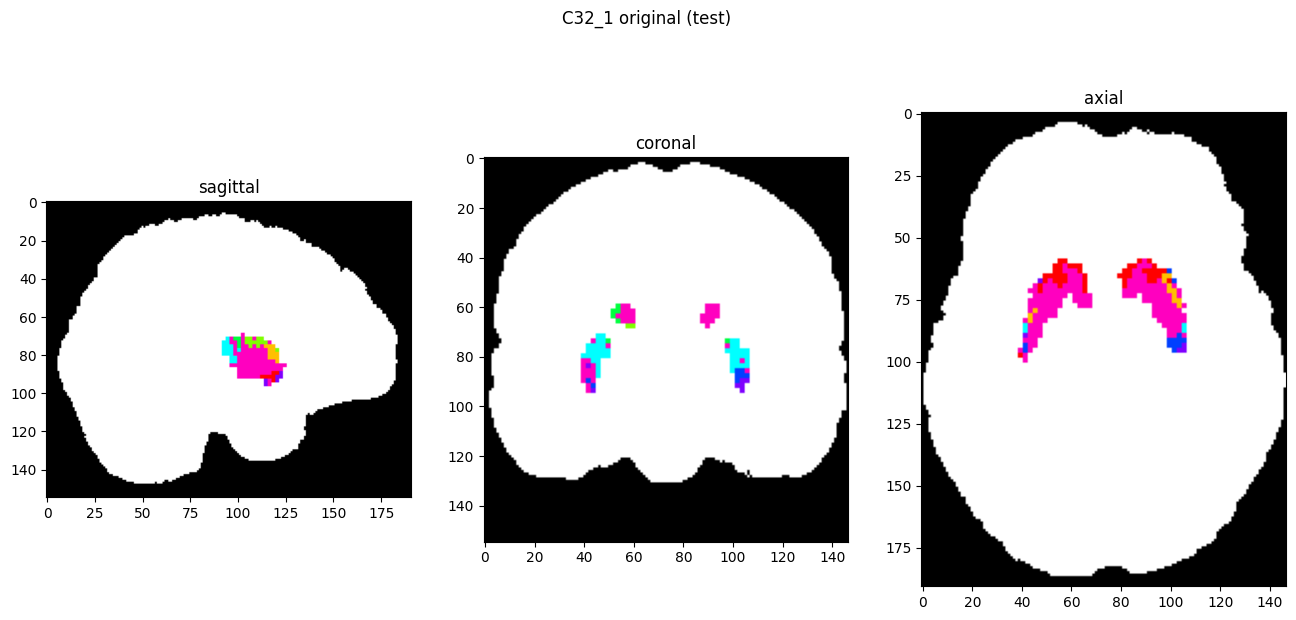
\includegraphics[width=0.9\textwidth]{con_test_o}
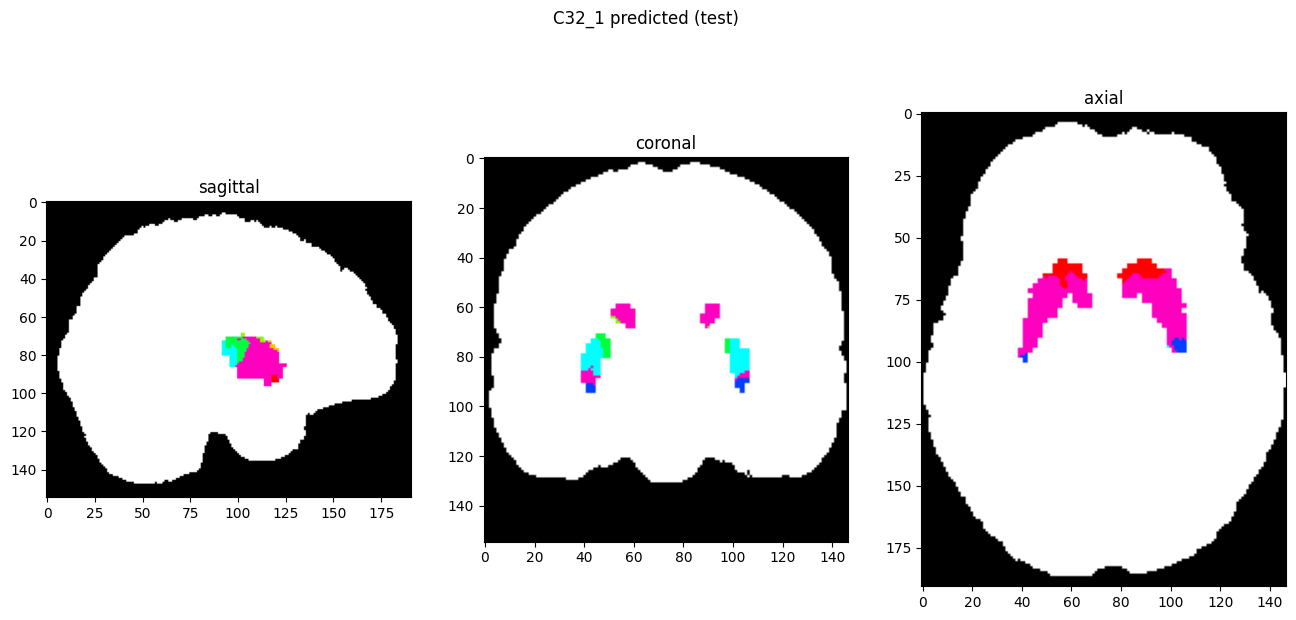
\includegraphics[width=0.9\textwidth]{con_test_p}
\caption{Test Predictions: Relative Connectivity}
\label{fig:pred-tes-con}
\end{figure}


